\chapter{Fundamentals and Related Work}

\section{Software-Defined Networking}

The origins of Software-Defined Networking (SDN) go back to as early as 1995, however the first implementations were only developed in 2001 and the promotion of SDN began with the foundation of the non-profit industry consortium Open Networking Foundation (ONF) in 2011. \cite{roadtosdn}
The ONF is dedicated to push open standards like OpenFlow into the industry and adapt them.
In this following section a brief overview of the SDN architecture and concepts, including the OpenFlow standard and Open vSwitch, is given.

\subsection{Motivation}

Today's internet is part of the modern society for private users, enterprises and vital infrastructure services. Networks are required to evolve in order to address the challenges that are entailed with new applications, services and a growing number of end-users.

With a more detailed view on the challenges of current network infrastructures one comes to see the following limitations: \cite{onfnewnorm}

\begin{itemize}
\item \textbf{Inability to scale}: With the expansion of data centers, networks grow too. Configuring and managing these additional network devices comes at a high administrative effort. With the virtualization of data-centers network traffic patterns become more and more dynamic and unpredictable. With multi-tenancy an additional complication is introduced, because different end-users and services need require distinct network characteristics. Network management and scaling of the architecture cannot be achieved with a manual configuration of the underlying infrastructure.
\item \textbf{Complexity}: In the past decades various new networking protocols have been adapted by the industry. To add or move a device, multiple of the already existing switches, routes and firewalls must be touched in order to manage and introduce new protocol-based mechanisms. With the virtualization of servers the amount of network interfaces that need connectivity is on the rise. The distribution of applications across a number of virtual machines are another demand that the current fairly static connections cannot adapt to.
\item \textbf{Inconsistent policies}: For IT departments to apply a network- or data center-wide policy, a lot of devices and mechanisms may need to be reconfigured. Virtual Machines can be created and rebuilt within no time, but if access or security rules need to be updated then the benefits of this dynamic can't be utilized to its full extent.
\item \textbf{Vendor dependence}: Standards are needed to match the requirements of the markets with the capabilities of networks and enable data center operators to customize the network to specific environments.
\end{itemize}

Traditionally, decisions about traffic-flows through the network are made directly by each network device, because the control logic and forwarding hardware are tightly coupled.

\subsubsection{Classical Switches \& Routers}

Packet forwarding (data plane) and routing decisions (control plane) in classical switching and routing are both within one device. The main components depicted in Figure 2.1 have the following functions:
\begin{enumerate}
\item The \textbf{forwarding path} typically handles data path operations for each packet. It generally consists of Application-Specific Integrated Circuits (ASIC), network-processors or general-purpose processors that forwards frames and packets at wire speed (line-rate). Their lookup functions can be further increased with memory resources like Content Addressable Memory (CAM) or Ternary Content Addressable Memory (TCAM) to contain the forwarding information.
\item The elements in the \textbf{control plane} are based on general-purpose processors that provide services like routing and signaling protocols, including ARP, MAC Learning and forwarding tables.
\end{enumerate}

\begin{figure}[H]
\centering

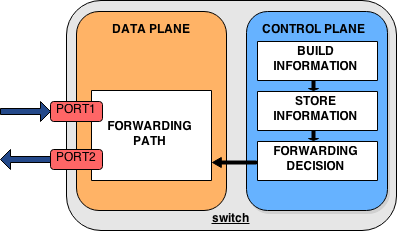
\includegraphics[width=0.5\textwidth]{images/fundamentals/switch_components}

\caption{"Classical" switch components}
\end{figure}

A switch consists of multiple ports for incoming and outgoing data. Internal forwarding tables classify the packets and forward them to one specific or multiple ports. It does so by collecting MAC addresses and storing their corresponding port in tables. Layer 2 switches also support the segregation into virtual LANs (VLAN), which enables the network operator to logically isolate networks that share a single switch.

Routers forward packets on the Network layer (Layer 3) and routing-decisions are made based on IP addresses. They contain a routing table wherein paths to neighbouring networks are stored, so that packets can be forwarded to their destination IP address. Other features that can be configured with routers are Quality of Service (QoS), Network Address Translation (NAT) and packet filtering.

The main differences between the classical architecture and SDN will be further described in the next section.

\subsection{Software-Defined Networking Concept}

SDN represents a novel dynamic, manageable, cost-effective and adaptable architecture \cite{onfdefinition} that is built to serve the dynamic infrastructures that are needed as a backbone for modern data centers. Opposed to the traditional approach, network control and forwarding functions are decoupled and thus can be programmed and divided into different applications and network services.
The work of the Open Networking Foundation laid out the OpenFlow standard as the base for modern SDN solutions.

\subsection{SDN Architecture}

SDN separates the architecture into three distinct layers that communicate with each other through different APIs. This separation is shown in Figure 2.2.

\begin{itemize}
\item \textbf{Infrastructure Layer:} here all physical and virtual devices (e.g. switches and routers) that are capable of the OpenFlow Protocol provide forwarding mechanisms on different Network Layers.
\item \textbf{Control Layer:} represents the 'network intelligence' and collects a global view of the network, by communicating with the switching elements through the so-called Southbound API.
\item \textbf{Application Layer:} consists of business applications that allow the network operator to extend the SDN controller on an abstracted level, without being tied to the actual details of the implementation of the infrastructure. This communication with the Control Layer is also called Northbound API.
\end{itemize}

\begin{figure}[H]
\centering

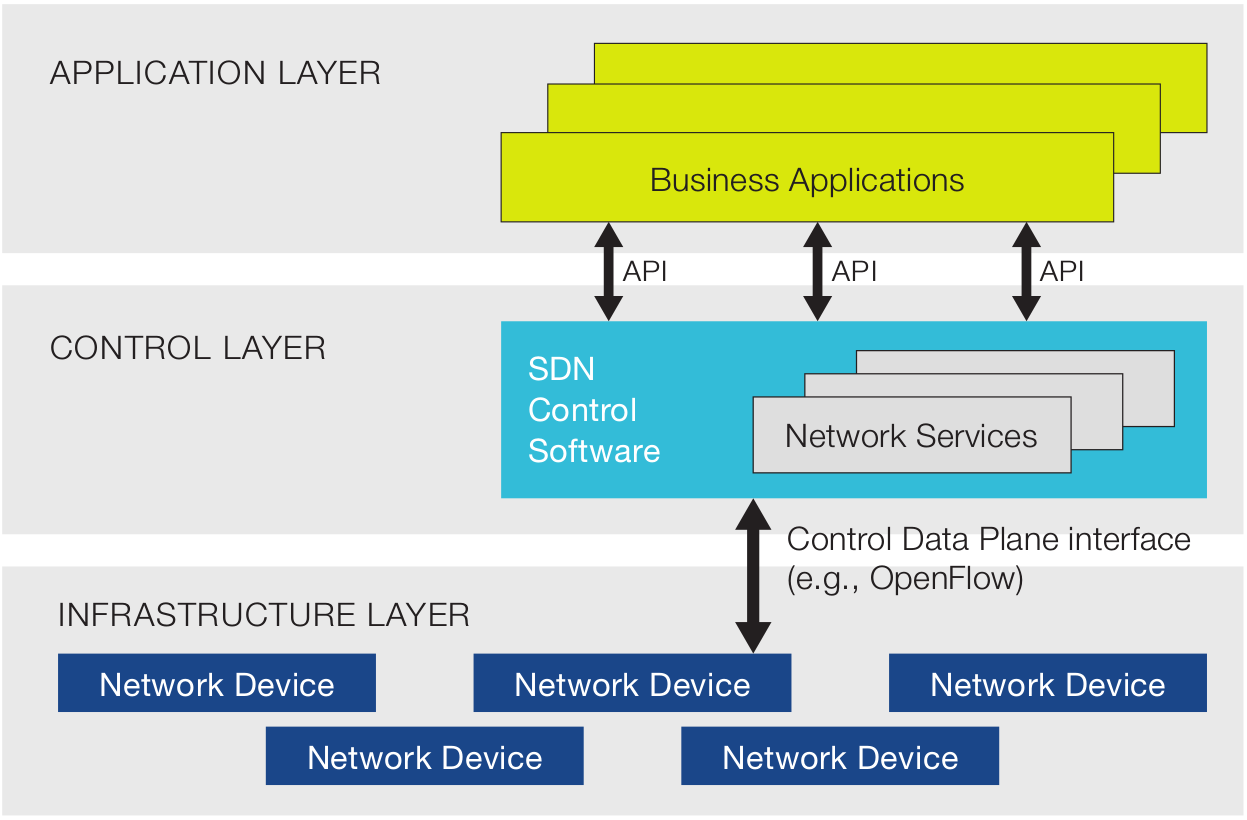
\includegraphics[width=0.5\textwidth]{images/fundamentals/sdn_logical_architecture.png}

\caption{SDN architecture}
\end{figure}

\subsection{OpenFlow}


With OpenFlow the Open Networking Foundation defined the first standard communications interface between the SDN architecture's control and forwarding layers. It enables manipulation and direct access to the forwarding plane of physical as well as virtual (hypervisor-based) network devices such as switches and routers. \cite{onfnewnorm}

\begin{figure}[H]
\centering

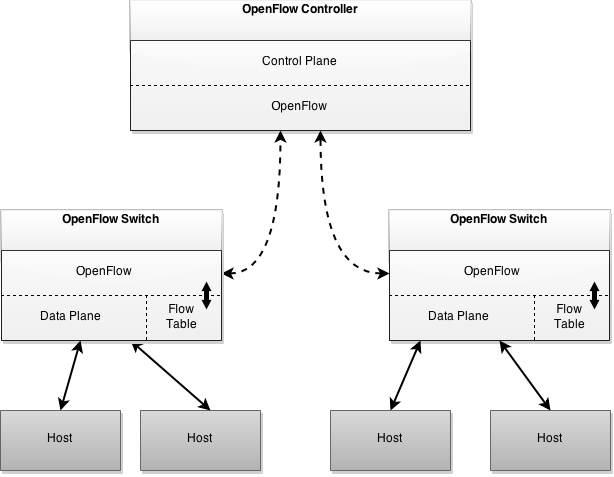
\includegraphics[width=0.6\textwidth]{images/fundamentals/openflow_architecture.png}

\caption{OpenFlow network architecture}
\end{figure}

OpenFlow first of all stands for the communications protocol that is used by SDN controllers to fetch information and configure switches. Additionally it is a switch specification with full support of OpenFlow.

Many of the OpenFlow-enabled switches and controllers up to today still solely support the OpenFlow version 1.0 (released in December 2009). The newest version at this date is 1.4, however the characteristics of OpenFlow in this work will focus on version 1.3, since it is the most recent specification which is supported by Open vSwitch.

The main features added since version 1.0 are, among others, support for VLANs, IPv6, tunnelling and per-flow traffic meters. \cite{ofversion13}

Generally the switches are backwards-compatible to version 1.0. In the following description the focus lies on the required features of all OpenFlow capable devices, however it has to be mentioned that some of them are optional features.

\subsubsection{OpenFlow Controller}

The OpenFlow controller is segregated from the switch and has two interfaces. The northbound interface is an API to the application layer for developing applications that control the network. The southbound interface connects with the underlying switches using the OpenFlow protocol.

\subsubsection{OpenFlow Switch}

There are two varieties of OpenFlow-compliant switches: \cite{ofspecification}
\begin{itemize}
\item \textbf{OpenFlow-only:} in these switches all packets are processed by the OpenFlow pipeline and have no legacy features.
\item \textbf{OpenFloy-hybrid:} support OpenFlow and normal Ethernet switching (including traditional L2 Ethernet switching, VLAN isolation, L3 routing, ACL and QoS). Most of the commercial switches that are available on the market today are of this type.
\end{itemize}

An OpenFlow switch includes one ore more flow tables and a group table, which have the function of carrying out packet lookups and forwarding. Another component is the OpenFlow channel that is connected to the external controller \cite{ofspecification}.

\begin{figure}[H]
\centering
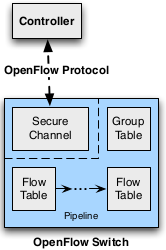
\includegraphics[width=0.3\textwidth]{images/fundamentals/openflow_switch_components.png}
\caption{OpenFlow switch components}
\end{figure}

Through the connection using the OpenFlow protocol, the controller is able to add, update and delete flow entries in Flow tables.  This action can be performed either reactively or proactively. Sets of flow entries are stored in each flow table and each flow entry consists of \textit{match fields}, \textit{counters}, and a set of \textit{instructions} used for matching packets.

Matching flow entries starts in the first flow table, however it may continue to additional flow tables. The first matching entry from each table is used and the instruction that is linked with that specific entry is performed. For packets without any matches a table-miss flow entry can be configured. Flow entries are usually forwarded to a physical port.

The instructions can either include actions or else modify the pipeline processing. Packet forwarding, packet modification and group table processing are available actions. Packets can be permitted to be sent to other tables with pipeline processing and additionally metadata can be exchanged between tables.

Packets can also be directed to a group, which contains a set of actions for flooding and more complex forwarding semantics (e.g. multipath, fast reroute and link aggregation).

\subsubsection{OpenFlow Ports}
OpenFlow ports are the network interfaces used for passing packets between OpenFlow processing and the rest of the network \cite{ofspecification}.
There are various types of ports that are supported by OpenFlow. This section will give a short overview about this port abstraction.
Incoming OpenFlow packets enter the switch on an ingress port, are then processed by the OpenFlow pipeline and forwarded to an output port. (See OF Tables figure for processing).

There are three types of OpenFlow ports that must be supported by an OpenFlow switch:
\begin{itemize}
\item \textbf{Physical ports:} are hardware interfaces on a switch.
\item \textbf{Logical ports:} don't directly interact  with a hardware interface.
\item \textbf{Reserved ports:} contain generic forwarding actions (e.g. sending to the controller, flooding or forwarding using traditional switch processing)
\end{itemize}

\subsubsection{OpenFlow Tables}

\textbf{\underline{Pipeline Processing}}

The OpenFlow pipeline specifies how packets correspond with each of the flow tables \cite{ofspecification}. 

\begin{figure}[H]
\centering
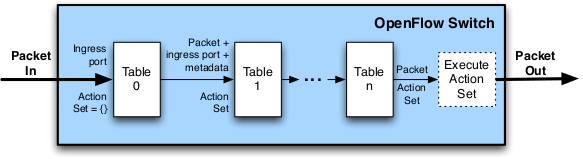
\includegraphics[width=0.8\textwidth]{images/fundamentals/openflow_pipeline_processing.png}
\caption{OpenFlow pipeline processing}
\end{figure}

As illustrated in the figure, each packet is matched against the flow entries starting at the first flow table, called flow table 0. The outcome of the match then decides if other of the sequentially numbered tables may be used. In the following sections the components of the Flow table, the matching procedures and different instructions will be described.


\textbf{\underline{Flow Table}}

A flow table contains flow entries, each of which consist of the following fields \cite{ofspecification}: 

\begin{table}[H]
\centering

\begin{tabular}{|c|c|c|c|c|c|}
\hline Match Fields & Priority & Counters & Instructions & Timeouts & Cookie \\ 
\hline 
\end{tabular} 

\caption{Fields within a Flow table}
\end{table}

\begin{itemize}
\item \textbf{match fields:} ingress port, packet headers and optionally metadata
\item \textbf{priority:} sets the priority of the flow entry
\item \textbf{counters:} is updated for matching packets
\item \textbf{instructions:} to alter the action set or pipeline processing
\item \textbf{timeouts:} set maximum amount of time or idle time before expiration of the flow
\item \textbf{cookie:} is an opaque data value chosen by the controller
\end{itemize}

Each flow table entry is uniquely identifiable by its match fields and priority. 


\underline{\textbf{Packet Matching}}

\begin{figure}[H]
\centering
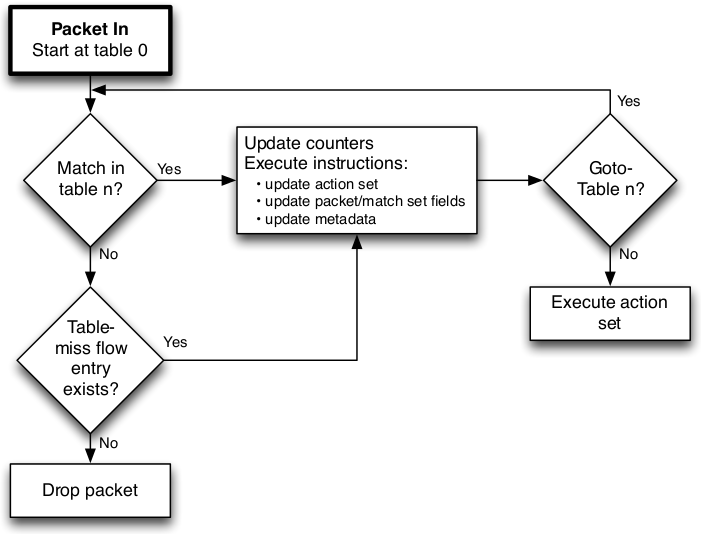
\includegraphics[width=0.6\textwidth]{images/fundamentals/openflow_packet_matching.png}
\caption{Packet flow through an OpenFlow switch}
\end{figure}

Upon a packet's arrival at the Flow Table, the packet match fields are extracted and used for the table lookup \cite{ofspecification}. They include different packet header fields. Additionally the ingress port can be matched with metadata fields.
If the values in the packet match fields are equal, then only the flow entry with the highest priority is selected. Furthermore the associated counters are updated and the instruction set is applied.

When the instruction set associated with a matching flow entry does not specify a next table, the pipeline processing stops. Only then the packet is processed with it's action set and in most cases forwarded as shown on the right-hand side of Figure 2.6.
However, if the lookup phase does not match any of the entries, a table-miss event occurs.


\underline{\textbf{Table-miss}}

Each flow table must support a table-miss flow entry which specifies how to process packets that are unmatched by other flow entries. The instructions associated with this entry are very alike to any other flow entries. Packets are either forwarded to other controllers, dropped, or it is continued with the next flow table. In case the table-miss flow entry is non-existent, unmatched packets are dropped by default. 


\underline{\textbf{Group Tables}}

A group table consists of group entries and it provides a way to direct the same set of actions as part of action buckets to multiple flows. A flow entry is pointed to a group and enables additional methods of forwarding (e.g. broadcast or multicast).


\underline{\textbf{Meter Tables}}

Meters are on a per-flow level and allow OpenFlow to implement various QoS operations, such as rate-limiting, but it can also be combined with per-port queues to implement more complex QoS like DiffServ.

The main components of a meter entry in the meter table are:

\begin{table}[H]
\centering

\begin{tabular}{|c|c|c|}
\hline Meter Identifier & Meter Bands & Counters \\ 
\hline 
\end{tabular} 

\caption{Fields within a meter entry in the meter table}
\end{table}

\begin{itemize}
\item \textbf{meter identifier:} a 32 bit unsigned integer uniquely identifying the meter
\item \textbf{meter bands:} each meter band specifies the rate of the band and the action that is triggered by exceeding the limit
\item \textbf{counters:} is updated when packets are processed by the meter
\end{itemize}

The rate of packets assigned to a meter are measured and controlled. Meters are directly attached to flow entries, as opposed to queues that are attached to ports. A meter is able to have one or more meter bands, each of which specifies the rate and the way packets should be handled. If the current measured meter rate reached the rate-limit, the band applies an action. 

A meter band is identified by its rate and consists of the following fields:

\begin{table}[H]
\centering

\begin{tabular}{|c|c|c|c|}
\hline Band Type & Rate & Counters & Type specific arguments \\ 
\hline 
\end{tabular} 

\caption{Fields within a meter band}
\end{table}

\begin{itemize}
\item \textbf{band type:} defines how the packets are processed
\item \textbf{rate:} selects the meter band for the meter and defines the lowest rate at which the band can apply
\item \textbf{counters:} is updated when packets are processed by the meter
\item \textbf{type specific arguments:} some bands have optional arguments
\end{itemize}

\begin{figure}[H]
\centering
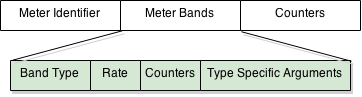
\includegraphics[width=0.6\textwidth]{images/fundamentals/openflow_qos.png}
\caption{OpenFlow QoS as a meter}
\end{figure}


\underline{\textbf{Instructions}}

Instructions are executed when a packet matches the flow entry \cite{ofspecification}. Their result is either a change to the packet, action set and/or pipeline processing. There are different instruction types and some of them are required for an OpenFlow-enabled switch whereas others are optional:

\begin{itemize}
\item \textbf{Meter \textit{meter\_id}:} Directs packet to the specified meter. The packet may be discarded as the result of the metering.
\item \textbf{Apply-Actions \textit{action(s)}:} Applies the specific action(s) instantly, without any change to the Action Set.
\item \textbf{Clear-Actions:} Immediately clears all the actions in the action set.
\item \textbf{Write-Actions \textit{action(s)}:} Merges the specified action(s) into the current action set.
\item \textbf{Write-Metadata \textit{metadata / mask}:} Writes the masked metadata value into the metadata field.
\item \textbf{Goto-Table \textit{next-table-id}:} Indicates the next table in the processing pipeline.
\end{itemize}

A maximum of one instruction of each type is associated with a flow entry and they are executed in the order as specified by the given list. Flow entries can also be rejected if the switch is not able to execute its instruction.


\underline{\textbf{Action Set}}

An action set is associated with each packet, which is empty by default \cite{ofspecification}. The action set can be modified using a \textit{Write-Action} or a \textit{Clear-Action} instruction. If there is no \textit{Goto-Table} instruction within the instruction set of a flow entry the pipeline processing is halted and the actions in the action set of the packet are executed.


\underline{\textbf{Actions}}

The following action types are available on OpenFlow-enabled switches \cite{ofspecification}:
\begin{itemize}
\item \textbf{Output:} A packet is forwarded to a specified OpenFlow port.
\item \textbf{Set-Queue:} Sets the Queue ID for a packet. This ID helps determining which Queue is used for scheduling and forwarding the packet. This forwarding behavior allows to enable basic QoS support on a port.
\item \textbf{Group:} Process the packet through the specified group.
\item \textbf{Push-Tag/Pop-Tag:} The ability to push/pop tags such as VLAN.
\item \textbf{Set-Field:} Modifies the values of header fields in a packet.
\item \textbf{Change-TTL:} Set the values of IPv4 TTL, IPv6 Hop Limit or MPLS TTL in a packet.
\end{itemize} 

\subsection{Open vSwitch}

\subsubsection{Concept \& Functionality}

Open vSwitch (OVS) is an open source software switch that is used in virtualized server environments. It is able to forward traffic between virtual network interfaces (e.g. connected to Virtual Machines) and the physical network, as well as between different VMs on the same physical host. It can be controlled using OpenFlow and the OVSDB management protocol. It can run on any Linux-based virtualization platform i.e. KVM, VirtualBox, XEN, ESXi and is part of the mainline kernel as of Linux 3.3 but can be run on kernel 2.6.32 and newer \cite{ovs-faq}.

OVS supports the following features \cite{ovs-readme}:
\begin{itemize}
\item 802.1Q VLAN model
\item Link Aggregation Control Protocol (LACP)
\item GRE and VXLAN tunneling
\item fine-grained QoS control
\item OpenFlow
\item per VM interface traffic policing
\item High-performance forwarding using a Linux kernel module
\end{itemize}

The internals of OVS are as follows \cite{prognetworkingovs}:

\begin{figure}[H]
\centering
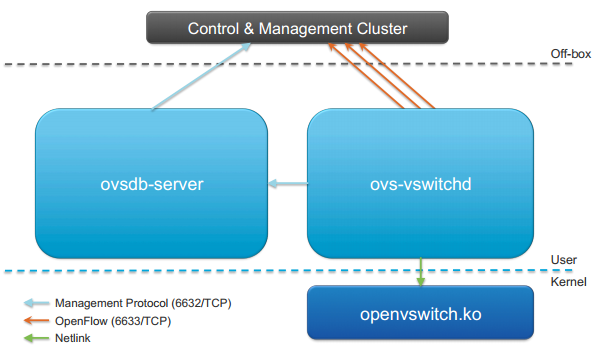
\includegraphics[width=0.6\textwidth]{images/fundamentals/openvswitch_architecture.png}
\caption{Architecture of Open vSwitch: kernelspace / userspace separation}
\end{figure}

The daemon which implements the switch is \textit{ovs-vswitchd} and is shipped with an additional Linux kernel module for flow-based switching that it communicates with using the netlink protocol \cite{ovsdeepdive}. The configuration for the switch is queried from a lightweight database server named \textit{ovsdb-server}.
Generally the decision about how a packet is processed is made in userspace, yet all following packets hit the cached entry in the kernel.

It is also possible to run the switch entirely in userspace, but it decreases the performance drastically.


\subsubsection{OVSDB}

Each Open vSwitch daemon has a database (OVSDB) that holds it's configuration \cite{ovsdbmanual}. The database is divided into multiple different tables with different purposes, with the ones related to this work outlined below:
\begin{itemize}
\item \textbf{Open\_vSwitch}: Open vSwitch configuration
\item \textbf{Port}: Port configuration
\item \textbf{Interface}: A physical network device within a Port
\item \textbf{QoS}: Quality of Service configuration
\item \textbf{Queue}: Output queue for QoS
\item \textbf{Controller}: OpenFlow controller configuration
\item \textbf{Manager}: OVSDB management connection
\end{itemize}


\subsubsection{Open vSwitch Management}

Multiple different configuration utilities exist for OVS, however only ovs-vsctl is explained in this section. It is used for querying and updating the configuration of the switch through interaction with the ovsdb-server.

\begin{figure}[H]
\centering
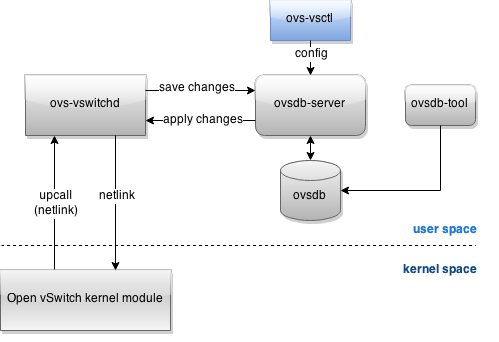
\includegraphics[width=0.6\textwidth]{images/fundamentals/openvswitch_vsctl.png}
\caption{Visualization of the ovs-vsctl tool's components}
\end{figure}

The tool also configures ovs-vswitchd and can be seen as a high-level interface for the database.
The commands below are available for the OVS configuration that is needed to get a basic network setup running:

\begin{lstlisting}[language=commands]
$ ovs-vsctl add-br %bridge%
$ ovs-vsctl add-port %bridge% %port%
$ ovs-vsctl list-ports %bridge%
$ ovs-vsctl set Interface %port%
\end{lstlisting}

In order to add Flow entries to a bridge the \textit{ovs-ofctl} is needed. The default Flow entry contains the following parameters:

\begin{lstlisting}[language=commands]
$ ovs-ofctl add-flow br-int hard_timeout=0,idle_timeout=0,priority=1,actions=normal
\end{lstlisting}


\subsubsection{QoS}

With Open vSwitch Quality of Service can be configured for ports that virtual machines are connected to. The minimal and maximal rate-limits can be defined in bit / s and applied to a queue. With the use of this feature the network traffic from the switches internal bridge to a virtual network interface can be shaped (egress).

\begin{figure}[H]
\centering
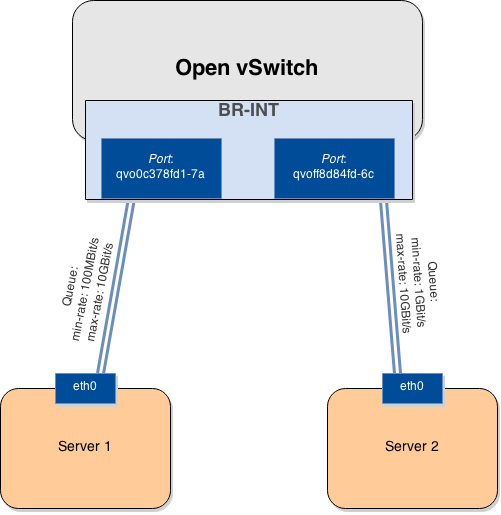
\includegraphics[width=0.5\textwidth]{images/fundamentals/openvswitch_qos-queues.png}
\caption{QoS Queues attached to a Port in OVS}
\end{figure}

The approach used in this work does not modify the OF Flow and their actions, which means that all Queues on a OVS are within the same Flow entry. The QoS port assurances in OVS make use of the 'tc' implementation which is included in the Linux kernel.



% % http://linux.die.net/man/8/tc % %
% % http://linux.die.net/man/8/tc-htb % %
% % http://www.istudies.net/journal/sites/default/files/Extended%20Linux%20HTB%20Queuing%20Discipline%20Implementations.pdf % %
% %https://github.com/stanzgy/nova-network-qos/blob/master/nova-network-qos-intro.rst % %
% %http://luxik.cdi.cz/~devik/qos/htb/manual/userg.htm % %
Traffic control (tc) uses 'queuing discipline' (qdisc) for configuring the network interface \cite{tc-manual}. They are the fundamental schedulers used under Linux. When a packet is sent, it is enqueued to the qdisc for the interface and shortly after the kernel is trying to get as many packets as it can from the qdisc, so they can be forwarded to the network adaptor driver. By default the 'pfifo\_fast' qdisc is set in the kernel, which is a pure 'First In, First out' queue.

When setting QoS in OVS a classful qdisc named Hierarchy Token Bucket (HTB) is used. HTB is meant as a more understandable, intuitive and faster replacement for the Class Based Queuing (CBQ) qdisc in Linux \cite{htb-guide}. It helps to control the use of the outbound bandwidth on a given link. 

For further understanding the following graph shows a HTB tree that contains on qdisc root and two classes (leaves) with different configurations:

\begin{figure}[H]
\centering
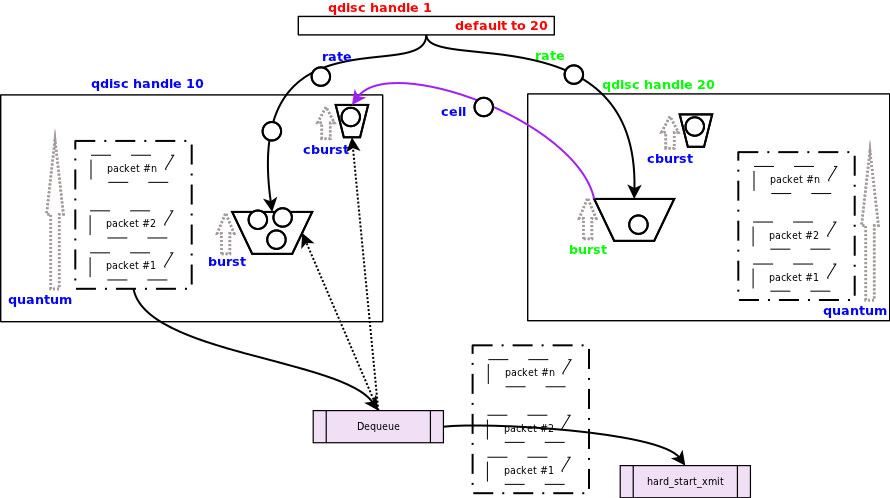
\includegraphics[width=0.7\textwidth]{images/fundamentals/htb_qdisc.png}
\caption{HTB: qdisc classes linked together as a tree} \cite{htb-qdiscs} 
\end{figure}

The terminology that is used for defining HTB classes is as follows:
\begin{itemize}
\item \textbf{burst:} the size of the token bucket
\item \textbf{rate:} the speed at which tokens are generated and put in the bucket (in the leaf)
\item \textbf{quantum:} the amount of bytes to serve from a single leaf at once
\item \textbf{ceil:} the definite upper class rate (this is the value that is set by the maximal rate defined in OVS QoS)
\item \textbf{cburst:} the burst for ceil (gets computed)
\end{itemize}

This tree was created using the following commands:
\begin{lstlisting}[language=commands]
$ tc qdisc add dev eth0 root handle 1: htb default 20
$ tc class add dev eth0 parent 1:0 classid 1:10 htb rate 200kbit ceil 400kbit prio 1 mtu 1500
$ tc class add dev eth0 parent 1:0 classid 1:20 htb rate 200kbit ceil 200kbit prio 2 mtu 1500
\end{lstlisting}

In figure 2.11 a root named 'qdisc handle 1' which applies filters to decide the direction of packets is depicted. It includes two leaves: 'qdisc handle 10' and set as default another leaf named 'qdisc handle 20'.

With the above listed commands the leaves were configured with the following parameters:

\begin{table}[H]
\centering

\begin{tabular}{|c|c|c|}
\hline Leaf parameter & \#10 & \#20 \\ 
\hline Rate value & 200 KBit/s & 200 KBit/s \\ 
\hline Ceil value & 400 KBit/s & 200 KBit/s \\ 
\hline Priority & 1 & 2 \\ 
\hline 
\end{tabular} 

\caption{Qdisc leaf configuration}
\end{table}

The difference between the rate and ceil value in leaf \#10 means it can borrow 200 KBit/s more than it's actual rate, while leaf \#20 cannot because its rate value equals the ceil value.

The HTB leaves always match one of the following three statuses \cite{htb-qdiscs}:
\begin{itemize}
\item \textbf{HTB\_CAN\_SEND:} the class can send using its own tokens
\item \textbf{HTB\_CANT\_SEND:} the class can't send nor borrow and no packets are permitted to leave the class
\item \textbf{HTB\_MAY\_BORROW:} the class can't send using its own tokens, but can try to borrow from another class
\end{itemize}

When a group of packets enters \textit{tc} that are marked with the flag \#10 and are directed to it, however the bucket does not contain enough tokens to let the first packets through then it will try to borrow tokens from leaf \#20. The quantum value defines the maximal amount that leaf \#10 will try to send at once. It is 1500 bytes, as that is the default MTU. If the first packet has a size of 1400 bytes and the bucket in leaf \#10 has enough tokens for 1000 bytes it will try to borrow the remaining 400 bytes from the neighbor leaf. The quantum value can be used to privilege a leaf compared to others, because it specifies the tokens that it can borrow from other leaves in the tree.

By configuring \textit{tc} the quantum value is not directly managed. It is automatically calculated based on an intermediary parameter named \textit{r2q} with the following formula:  $ quantum = \frac{rate}{r2q} $ This value is set on the root qdisc and is used across all of its leaves. Its default value is set to 10.


\subsubsection{VXLAN}

Virtual Extensible LAN tunnels are used with Open vSwitch in this work to encapsulate isolated layer 2 network traffic between compute nodes. The benefits of VXLAN are that it can adress up to 16M tenant networks as opposed to the 4K in VLAN, it allows for better scaling and because the VXLAN support is only required at the endpoints of the tunnels it permits a vendor flexibility \cite{openstack-vxlan}. The tunnels can be used to perform a large scale isolation within a network.


\section{Cloud Computing Infrastructures}
% Call it Infrastructure-as-a-Service? %


\subsection{OpenStack}

The OpenStack project was founded by Rackpace Cloud and NASA, however up to this day  more than 200 companies are contributing to it.
With OpenStack it is possible to design, deploy and maintain a private or public cloud installation. It is a flexible, scalable and open-source approach that combines multiple technologies into one Infrastructure-as-a-Service (IaaS) \cite{openstack-ops}. All of the interrelated services include an API that offers administrators different ways of controlling the cloud, be it through a web-interface, a command-line client or a Software Development Kit. All of the core components that are part of OpenStack are implemented in Python.


\textbf{Conceptual architecture}

The following graph shows the interaction between different OpenStack services that are involved in launching a virtual machine.

\begin{figure}[H]
\centering
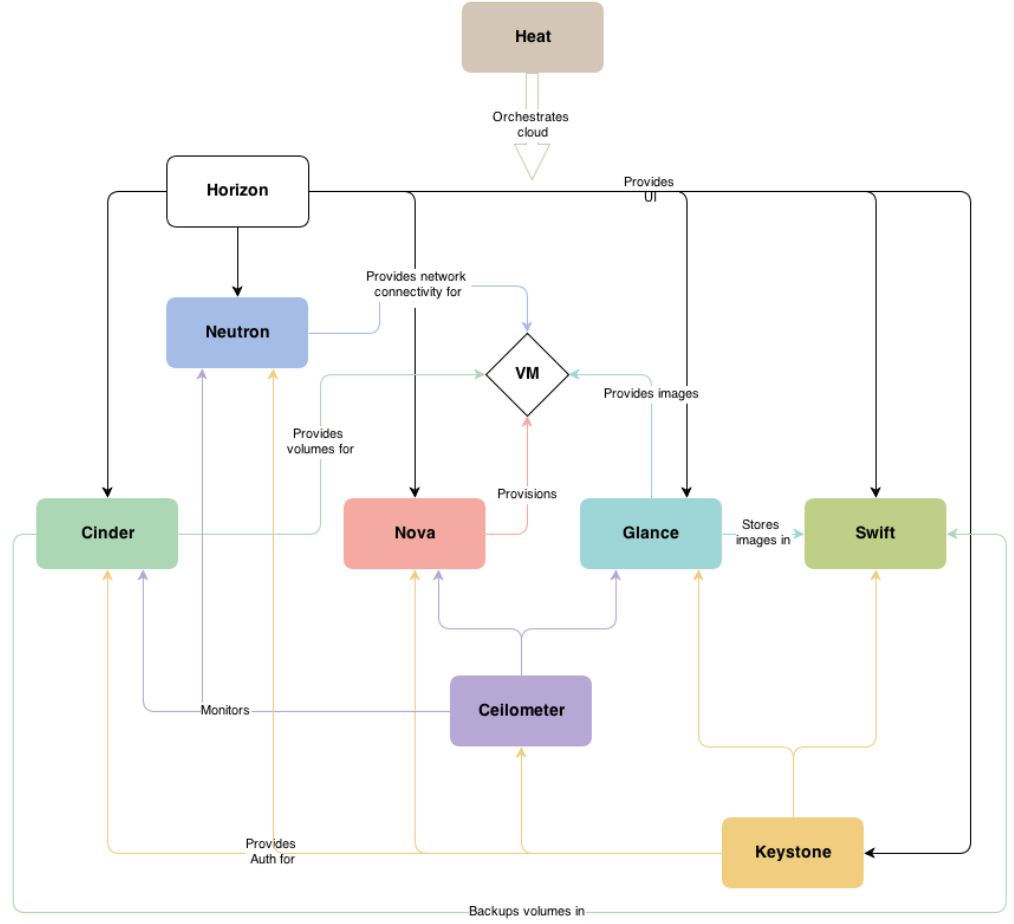
\includegraphics[width=0.8\textwidth]{images/fundamentals/openstack_conceptual_arch.png}
\caption{Interaction among OpenStack services}\cite{openstack-installjuno}
\end{figure}


\subsection{OpenStack Compute (Nova)}

Nova is used to provision and manage large amounts of virtual machines . It supports different hypervisors and the number of physical hosts running the compute services can be scaled horizontally with no requirement of hardware resources from specific vendors. Hosts that provide Nova services are also called 'Compute Nodes'. Data center can be divided into so called tenants, which are isolated users with their own servers, security groups and externally reachable IP addresses (Floating IP addresses). 

\begin{figure}[H]
\centering
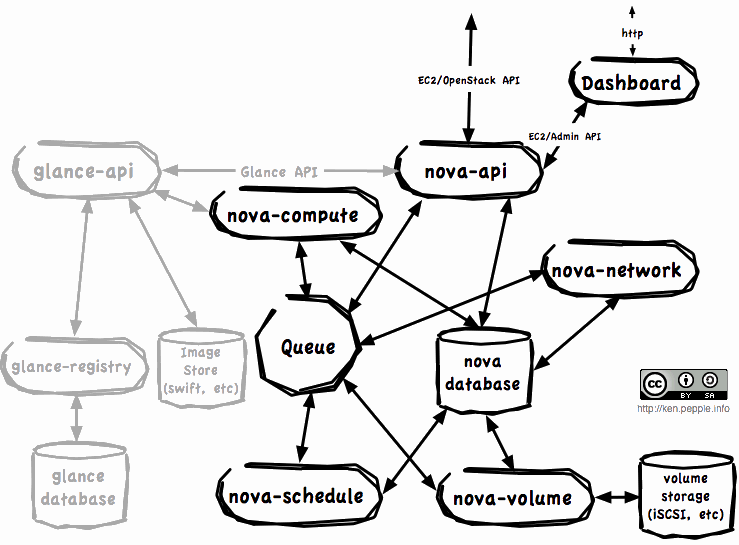
\includegraphics[width=0.5\textwidth]{images/fundamentals/openstack_nova.png}
\caption{OpenStack Compute service} \cite{nova-arch}
\end{figure}

\textbf{Compute Node segregation}

An OpenStack cloud can be logically and physically grouped on different levels \cite{openstack-ops}:
\begin{itemize}
\item \textbf{Region:} A Region has its own full OpenStack deployment and can be physically at a different location. Regions share a set of Keystone and Horizon services to provide access control and the graphical management interface.
\item \textbf{Availability Zone:} Inside of a Region, it is possible to logically group multiple compute nodes into Availability Zones. This zone can be specified when new servers or stacks (via Heat) are instantiated.
\item \textbf{Host Aggregates:} Compute nodes can also be logically grouped into Host Aggregates by using meta-data to tag them. This feature can be used to separate nodes with certain hardware characteristics (e.g. with SSD drives) from others.
\end{itemize}

For zoning compute nodes availability zones will be used in the Connectivity Manager in order to achieve the best networking performance between individual servers.

\textbf{Default VM Placement}

Nova makes use of the nova-scheduler service in order to regulate on which host a new VM is launched. The nova-scheduler interacts with other components through the queue and central database repo. All of the compute nodes periodically send an update about their status,  available resources and hardware capabilities to the nova-scheduler. It collects this data to make a decision about the placement based on a filter scheduler which takes the following criteria into account:
\begin{itemize}
\item are within the requested availability zone
\item have sufficient RAM available
\item are capable of servicing the request
\end{itemize}
By default Nova allows its RAM and vCPU resources to be overcommited, which means that more than the physically available resources can be deployed. However this is to the detriment of their performance.

\subsection{OpenStack Orchestration (Heat)}

Heat provides a template-based orchestration service for creating and managing cloud resources. This means multiple OpenStack resource types (such as virtual machines, floating IP addresses, volumes, security groups and users) can be generated and also maintained with additional functionality like auto-scaling.


\subsection{OpenStack Neutron}
% % PDF: Performance of Network Virtualization in CCI % %

In the early versions of OpenStack, virtual networking was exclusively a sub-component of Nova called Nova-network. This service has its limitations, because it is closely coupled with networking abstractions and no API available. With Neutron the implementation is decoupled from the network abstraction and it provides a flexible management interface to administrators and users.


\subsubsection{Networking Concepts}

Neutron is responsible for defining network connectivity and addressing within OpenStack. In the main network abstraction the following components are defined:
A network as a virtual layer 2 segment, a subnet as a layer 3 IP address space used within a network, a port as an interface to a network or subnet, a router that performs address translation and routing between subnets, a DHCP server responsible for IP adress distribution, a security group for filtering rules acting as a cloud firewall and Floating IP addresses to give VMs external network access.

Neutron exposes an extensible set of APIs for creating and administering its components. Neutron consists of the following elements \cite{openstack-training}:
\begin{itemize}
\item \textbf{neutron-server:} Provides the logic for SDN, however it does not contain any of its functionality in itself. It provides a generic API for the network operations, is modular and extended with the following agents.
\item \textbf{L2 agent:} Plugin-specific agent that manages networking on a compute node. For more details, see Modular Layer 2 section.
\item \textbf{DHCP agent:} Provides DHCP services to tenant networks through dnsmasq instances.
\item \textbf{L3 agent:} Provides L3/NAT forwarding to allow external network access for VMs (virtual routers).
\item \textbf{Metadata agent:} Acts as a proxy to the metadata service of Nova.
\end{itemize}

The different agents can interact with the neutron-server process through a message queue and the OpenStack Networking API. In most use-cases the neutron-server and the different agents can run on the controller node or on a separate network controller node, with the plugin agent running on each compute node.


\subsubsection{Modular Layer 2}

The ML2 plugin is a framework that allows the simultaneous usage of multiple layer 2 networking technologies. It also helps vendors develop new agents, because an abstract method for their services is already specified.

\begin{figure}[H]
\centering
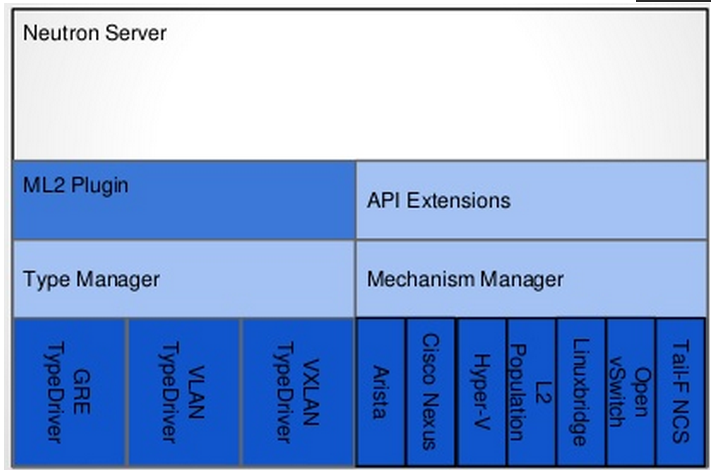
\includegraphics[width=0.3\textwidth]{images/fundamentals/neutron_ml2.png}
\caption{Neutron modular framework, including ML2 drivers}
\end{figure}

The plugin integrates the type driver and the mechanism driver. The type driver defines the network types that can be declared when a new network is created and currently includes: local, flat, vlan, gre and vxlan. The mechanism driver enables the mechanism for accessing these network types, i.e. Open vSwitch, Linux Bridge or other vendor-specific solutions. 



\textbf{ML2: Open vSwitch}

Open vSwitch is the ML2 mechanism driver that is set as default when installing OpenStack with Neutron enabled using the devstack script. It is also the most commonly deployed agent.

\begin{figure}[H]
\centering
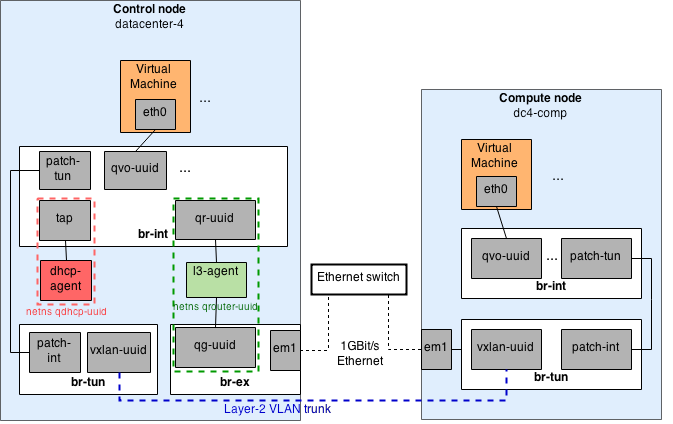
\includegraphics[width=0.7\textwidth]{images/fundamentals/neutron_ovs_bridges.png}
\caption{Neutron with OVS and VXLAN enabled}
\end{figure}

The above figure shows the connectivity of a VM, which has a 'qvo'-Port located in the internal bridge of the OVS. Each network within Neutron has its own network namespace and the external gateway uses the 'qrouter' namespace for routing. The connection between the compute nodes in this example uses VXLAN as the network type driver.


\subsubsection{Network Distinction}

Neutron is connected to different networks. For internet routable connections the external network is used. The management network is created by the network operator and is mapped to pre-existing networks within the datacenter, which is used to connect the different hosts. The tenants within OpenStack have their own isolated self provisioned private networks. Those can optionally be connected to other tenant or external networks. The abstraction of those tenant networks is possible through network namespaces. This allows overlapping IP addresses within the datacenter.


\subsubsection{Neutron Workflow}

From the time when Neutron is started as a process within the OpenStack controller node to booting a virtual machine, it passes through the following steps:

\begin{enumerate}
\item Start Neutron-Server
\item Start Open vSwitch Agent
\item Start L3-Agent
\item Start DHCP-Agent
\item Start Metadata-Agent
\item Create Networks
\item Create Routers
\item Boot VMs
\end{enumerate}

Once the VM is started it has full network connectivity within the tenants network and if a floating IP address was attached to it, then it can also be reached from the internet.

%\textbf{Neutron - Nova interaction}
%
%\begin{enumerate}
%\item Request: Create VM connected to network X (API)
%\item Create VM (RPC: Nova API to Nova conductor)
%\item Nova schedules VM
%\item Create VM (RPC: Nova conductor to Nova compute)
%\item Create Port (API: Nova compute to Neutron service)
%\item Create tap device
%\item Notify L2 agent (RPC)
%\item get\_device\_details (RPC: L2 agent to Neutron service)
%\item Configure local VLAN, OVS flows
%\item Send port\_up notification (RPC: L2 agent to Neutron service)
%\item Send port\_up notification (API: Neutron service to Nova)
%\item port\_up (RPC: Nova service to Nova compute)
%\item Nova compute boots VM
%
%\end{enumerate}


\section{Conclusion}

This chapter laid out the technological fundamentals for this thesis. Starting with the motivation for the use of SDN and the difference to the traditional networking approach and going on to describe the OpenFlow standard which forms the basis for the work of the Open Networking Foundation. The Open vSwitch makes full use of the OpenFlow standard and protocol and forms the basis for the network switching infrastructure used in this thesis. Furthermore it provides the service for enabling network traffic shaping which is described on a deep technical level. All necessary components that are used in connection to this work are introduced.